% =====================================
% COURS : POLYNOMES DU SECOND DEGRE
% Niveau : 1ere Specialite
% =====================================

% Section I : Les polynomes
\section{Les polynômes}

% Definition des monomes
\begin{Definition}[Monômes]
    Les\voc{monômes} sont des expressions algébriques formées du produit d'un coefficient $a$ réel par une puissance (entière) d'une indéterminée $X$ : $aX^n$. 
    
    L'exposant de $X$ est appelé le\voc{degré du monôme}.

\end{Definition}

\begin{Exemple}[Exemples de monômes]
    \begin{tcbenumerate}[3]
        \tcbitem $4X^0=4$ est de degré $0$
        \tcbitem $-3X^1=-3X$ est de degré $1$
        \tcbitem $\pi X^2$ est de degré $2$
        \tcbitem $12{,}5X^7$ est de degré $7$
        \tcbitem $0X=0$ est de degré $-\infty$
    \end{tcbenumerate}
\end{Exemple}

% Definition des polynomes
\begin{Definition}[Polynôme]
    Un\voc{polynôme} est une somme (finie) de monômes.
    
    \begin{itemize}
        \item Un polynôme est dit\voc{réduit} lorsque tous ses monômes sont de degrés distincts.
        \item Le\voc{degré d'un polynôme réduit} est le plus grand degré de ses monômes.
        
        \item Un polynôme réduit est dit\voc{ordonné} lorsque ses monômes sont rangés suivant les puissances décroissantes de l'indéterminée $X$.
        
    \end{itemize}
\end{Definition}

\begin{Exemple}[Polynômes]
    \begin{tcbenumerate}
        \tcbitem $-3+8X^2+4X-7X^3-7X+10$ est un \acc{polynôme}.
        \tcbitem $3X^2-12X^5 +2$ est sous forme réduite mais $5+7X-14X^2+8X$ n'est pas sous forme \acc{réduite} car les monômes $7X$ et $8X$ sont semblables (même degré).
        \tcbitem $-7X^3+X-3$ est \acc{ordonné} alors que $X-7X^2+2$ ne l'est pas.
    \end{tcbenumerate}
\end{Exemple}


% Remarque sur les applications
\begin{Remarque}[Applications des polynômes]
    Les polynômes ont ceci de merveilleux qu'ils peuvent s'appliquer à un très grand nombre d'objets. $X$ peut désigner des nombres bien sûr mais aussi des polynômes, des fonctions, des transformations géométriques, des tableaux de nombres (matrices), etc.
\end{Remarque}

% Section II : Differentes expressions et lien avec la courbe representative
\section{Differentes expressions et lien avec la courbe representative}

\subsection{La forme développée}

% Definition fonction polynome de degre 2
\begin{Definition}[Fonction polynôme de degré 2]
    Une\voc{fonction polynôme de degré 2} est une fonction $f$ définie sur $\R$ par 
    \begin{center}$f(x)=a x^2+b x + c$\end{center}
    avec $a\in \R^*$ et $b,c \in \R$.
    
    Cette écriture de $f(x)$ est appelée\voc{forme développée} de $f(x)$.
\end{Definition}

% Definition de la parabole
\begin{Definition}[Parabole]
    Soit $f$ une fonction polynôme de degré 2 définie sur $\R$ par $f(x)=a x^2+b x + c$, avec $a\in \R^*$ et $b,c \in \R$.
    
    \begin{itemize}
        \item Si $a>0$ alors la représentation graphique de $f$ est une\voc{parabole} $\mathcal{P}$ \frquote{tournée vers le haut}.
        \item Si $a<0$ alors la représentation graphique de $f$ est une \acc{parabole} $\mathcal{P}$ \frquote{tournée vers le bas}.
    \end{itemize}
    
    \begin{center} 
    \begin{tabular}{cc}
    \begin{tikzpicture}[scale=0.8]
        \draw[line width=1.2pt,color=monrose,smooth,samples=100,domain=-0.1:3.1] plot(\x,{(\x-1.5)^(2.0)+0.2});    
        % Axis
        \draw[thick,->] (-0.5,0) -- (3.5,0);
        \draw[thick,->] (0,0) -- (0,2.8);
        \node at (-0.2,2.4) {$c$};
    \end{tikzpicture}
    &
    \begin{tikzpicture}[scale=0.8]
        \draw[line width=1.2pt,color=monrose,smooth,samples=100,domain=-0.1:3.1] plot(\x,{-(\x-1.5)^(2.0)+2.7});    
        % Axis
        \draw[thick,->] (-0.5,0) -- (3.5,0);
        \draw[thick,->] (0,0) -- (0,2.8);
        \node at (-0.2,0.5) {$c$};
    \end{tikzpicture}
    \\ 
    $a>0$ & $a<0$ \\ 
    \end{tabular}  
    \end{center}
\end{Definition}

% Remarque sur le sommet et l'ordonnee a l'origine
\begin{Remarque}[Sommet et ordonnée à l'origine]
    \begin{itemize}
        \item Le point \frquote{le plus haut} ($a<0$) ou \frquote{le plus bas} ($a>0$) est appelé le\voc{sommet} de la parabole. 
        \item L'ordonnée du point de $\mathcal{P}$ qui a pour abscisse 0 est le coefficient $c$.
    \end{itemize}
\end{Remarque}

\subsection{La forme canonique}

% Propriete forme canonique
\begin{Propriete}[Forme canonique]
    Soit $f$ une fonction définie sur $\mathbb{R}$ par $f(x) = ax^{2} + bx + c$ une fonction polynôme du second degré ($a \neq 0$). 
    
    Il existe deux nombres réels $\alpha$ et $\beta$ tels que pour tout nombre réel $x$, on a :
    \begin{center}$ax^{2} + bx + c = a(x-\alpha)^{2} + \beta$\end{center}
    
    L'écriture $a(x-\alpha)^{2} +\beta$ est la\voc{forme canonique} de la fonction $f$.
    
    \begin{tcbenumerate}[2]
        \tcbitem[halign=center] $\alpha = -\dfrac{b}{2a}$
        \tcbitem[halign=center] $\beta = -\dfrac{b^2-4ac}{4a}$
    \end{tcbenumerate}
\end{Propriete}
\begin{Propriete}[Forme canonique]
    Soit $f$ une fonction définie sur $\mathbb{R}$ par $f(x) = ax^{2} + bx + c$ une fonction polynôme du second degré ($a \neq 0$). 
    
    Il existe deux nombres réels $\alpha$ et $\beta$ tels que pour tout nombre réel $x$, on a :
    \begin{center}$ax^{2} + bx + c = a(x-\alpha)^{2} + \beta$\end{center}
    
    L'écriture $a(x-\alpha)^{2} +\beta$ est la\voc{forme canonique} de la fonction $f$.
    
    \begin{tcbenumerate}[2]
        \tcbitem[halign=center] $\alpha = -\dfrac{b}{2a}$
        \tcbitem[halign=center] $\beta = -\dfrac{b^2-4ac}{4a}$
    \end{tcbenumerate}
\end{Propriete}
% Propriete sommet de la parabole
\begin{Propriete}[Sommet de la parabole]
    Soit $f$ une fonction polynôme de degré 2 de forme canonique $f(x) = a(x-\alpha)^{2} + \beta$.
    
    \begin{tcbenumerate}[2]
        \tcbitem Le\voc{sommet} de la parabole $\mathcal{P}$ a pour coordonnées $S(\alpha;\beta)$.
        \tcbitem La parabole $\mathcal{P}$ a pour\voc{axe de symétrie} la droite d'équation $x=\alpha$.
    \end{tcbenumerate}
\end{Propriete}
\newpage
% Propriete variations du trinome
\begin{Propriete}[Variations du trinôme]
    Soit $f$ une fonction définie sur $\mathbb{R}$ par $f(x) = ax^{2} + bx + c$ une fonction polynôme du second degré ($a \neq 0$) avec forme canonique $f(x) = a(x-\alpha)^{2} + \beta$.
    
    Les variations du trinôme $f$ sont données par les tableaux suivants :
    
    \begin{tcbenumerate}
        \tcbitem Si $a > 0$, la fonction $f$ est décroissante sur l'intervalle $\CrochetD-\infty;\alpha\CrochetD$ et croissante sur l'intervalle $\CrochetG\alpha ; +\infty\CrochetG$.
        
        \begin{center}
        \begin{tabular}{cc}
        \begin{tikzpicture}[scale=0.7]
            %Fonction    
            \draw[line width=1.2pt,color=monrose,smooth,samples=100,domain=-0.8:2.6] plot(\x,{0.8*(\x-1)^(2.0)+1})node [above] {$\mathcal{P}$};    
            % Point
            \draw[blue,very thick,dashed,-] (0,1) node[left] {\large{$\beta$}} -- (1,1) -- (1,0) node[below] {\large{$\alpha$}};   
            %Tangente
            \draw[blue,thick,<->] (0.5,1) -- (1.5,1);    
            % Axes
            \draw[thick,->] (-1.5,0) -- (3.5,0);
            \draw[thick,->] (0,-0.5) -- (0,4);
        \end{tikzpicture}
        &
        \begin{tikzpicture}
        \tkzTabInit{$x$/1,$f$/1.8}
        {$-\infty$,$\alpha$,$+\infty$}
        \tkzTabVar{+/$+\infty$,-/$\beta$,+/$+\infty$}
        \end{tikzpicture}
        \end{tabular}
        \end{center}
        
        \tcbitem Si $a < 0$, la fonction $f$ est croissante sur l'intervalle $\CrochetD-\infty;\alpha\CrochetD$ et décroissante sur l'intervalle $\CrochetG\alpha ; +\infty\CrochetG$.
        
        \begin{center}
        \begin{tabular}{cc}
        \begin{tikzpicture}[scale=0.7]
            %Fonction    
            \draw[line width=1.2pt,color=monrose,smooth,samples=100,domain=-0.8:2.6] plot(\x,{-0.8*(\x-1)^(2.0)+3})node [below] {$\mathcal{P}$};    
            % Point
            \draw[blue,very thick,dashed,-] (0,3) node[left] {\large{$\beta$}} -- (1,3) -- (1,0) node[below] {\large{$\alpha$}};   
            %Tangente
            \draw[blue,thick,<->] (0.5,3) -- (1.5,3);
            % Axes
            \draw[thick,->] (-1.5,0) -- (3.5,0);
            \draw[thick,->] (0,-0.5) -- (0,4);
        \end{tikzpicture}
        &
        \begin{tikzpicture}
        \tkzTabInit{$x$/1,$f$/1.8}
        {$-\infty$,$\alpha$,$+\infty$}
        \tkzTabVar{-/$-\infty$,+/$\beta$,-/$-\infty$}
        \end{tikzpicture}
        \end{tabular}
        \end{center}
    \end{tcbenumerate}
\end{Propriete}

\subsection{La forme factorisée}

% Propriete forme factorisee
\begin{EXO}{Forme factorisée à partir des racines}{}
Soit $f$ la fonction définie sur $\R$ par $f(x)=4x^2-20x-56$. On admet que les racines de $f$ sont $7$ et $-2$. \tcbitempoint{2} Déterminer la forme factorisée de $f$.

\begin{crep}
$f(x) = 4(x-7)(x+2)$
\end{crep}

\exocorrection

Les racines de $f$ sont $x_1 = 7$ et $x_2 = -2$.

La forme factorisée s'écrit $f(x) = a(x-x_1)(x-x_2)$ avec $a$ le coefficient dominant.

Dans la forme développée $f(x) = 4x^2-20x-56$, on lit $a = 4$.

Donc $f(x) = 4(x-7)(x-(-2)) = 4(x-7)(x+2)$.

\textbf{Vérification :} $4(x-7)(x+2) = 4(x^2+2x-7x-14) = 4(x^2-5x-14) = 4x^2-20x-56$ \checkmark
\end{EXO}

% Section III : Racine et signe d'un trinome
\section{Racine et signe d'un trinôme}

\subsection{Racine d'un trinôme}

% Definition des racines
\begin{Definition}[Racines d'un polynôme]
    Les\voc{racines} d'un polynôme sont les nombres réels qui \acc{annulent} ce polynôme.
    
    \begin{Remarque}[]
        Soit $f$ la fonction définie sur $\R$ par $f(x) = ax^2+bx+c$ avec $a \in \R^*$ et $b,c \in \R$. 
        

        Les \acc{racines} de la fonction polynôme $f$ sont les \acc{solutions} de l'équation $f(x)=0$. 


        Graphiquement, ce sont les abscisses des points d'intersections entre la courbe représentative de $f$, notée $\mathcal{C}_f$, et l'axe des \acc{abscisses}.
    \end{Remarque}
\end{Definition}

% Propriete racines et forme factorisee
\begin{Propriete}[Racines et forme factorisée]
    Si un polynôme est écrit sous \acc{forme factorieée} $a(x-x_1)(x-x_2)$ avec $a \neq 0$, alors ses \acc{racines} sont $x_1$ et $x_2$.\\

    De plus un polynôme de degré 2 est écrit sous forme développée $ax^2+bx+c$ et possède deux racines $x_1$ et $x_2$, alors :
    \begin{tcbenumerate}[2]
        \tcbitem La somme des racines est égale à $-\dfrac{b}{a}$
        \tcbitem Le produit des racines est égale à $\dfrac{c}{a}$
    \end{tcbenumerate}
\end{Propriete}

% Propriete somme et produit des racines
\input{Propriete/somme_produit_racines}

\subsection{Aspect graphique}

% Exemple aspect graphique des racines
\begin{Exemple}[Aspect graphique des racines]
    
    \begin{MultiColonnes}{3}
        \tcbitem[halign=center, valign=center] \definecolor{ffqqqq}{rgb}{1.,0.,0.}
    \definecolor{qqqqff}{rgb}{0.,0.,1.}
    \definecolor{ttqqqq}{rgb}{0.2,0.,0.}
    \begin{tikzpicture}[line cap=round,line join=round,>=triangle 45,x=1.0cm,y=1.0cm,scale=0.8]
    \draw[->,color=black] (-2.,0.) -- (3.,0.);
    \foreach \x in {-2.,-1.,1.,2.}
    \draw[shift={(\x,0)},color=black] (0pt,2pt) -- (0pt,-2pt) node[below] {\footnotesize $\x$};
    \draw[->,color=black] (0.,-2.5) -- (0.,3.);
    \foreach \y in {-2.,-1.,1.,2.}
    \draw[shift={(0,\y)},color=black] (2pt,0pt) -- (-2pt,0pt) node[left] {\footnotesize $\y$};
    \draw[color=black] (0pt,-10pt) node[right] {\footnotesize $0$};
    \clip(-2.,-2.5) rectangle (3.,3.);
    \draw[line width=1.2pt,color=ttqqqq,smooth,samples=100,domain=-2.0:3.0] plot(\x,{0-(\x)^(2.0)+(\x)+2.0});
    \draw [->,color=qqqqff] (2.805914536286458,0.8043788880386957) -- (2.1711777835787407,0.19016846006020638);
    \draw [->,color=ffqqqq] (-1.8740875019775842,0.8454315374971523) -- (-1.1410526494584565,0.1394736752707718);
    \begin{scriptsize}
    \draw[color=ttqqqq] (2,-2) node {\large{$\mathcal{C}_f$}};
    \draw[color=qqqqff] (2.8,1) node {\large{$x_{2}$}};
    \draw[color=ffqqqq] (-1.8,1) node {\large{$x_{1}$}};
    \end{scriptsize}
    \end{tikzpicture}
        \tcbitem[raster multicolumn=2]    Prenons la fonction $f$ définie sur $\R$ par $f(x)=-x^2+x+2$.
    \vspace{0.4cm}
    
    Sur cet exemple, on remarque que $\mathcal{C}_f$ coupe l'axe des abscisses en deux points.
    \vspace{0.4cm}
    
    De plus, on observe graphiquement les solutions $x_{1}$ et $x_{2}$ de l'équation $f(x)=0$, à savoir :
    \begin{center}$x_{1}=-1 \text{ et } x_{2} = 2$\end{center}
    Les racines du polynôme $-x^2+x+2$ semblent être $-1$ et $2$.
    \end{MultiColonnes}

\end{Exemple}

\subsection{Signe d'un trinôme donne sous forme factorisee}

% Methode etude de signe
\begin{Methode}[Étude de signe d'un trinôme donné sous forme factorisée]
    Pour étudier le signe d'un polynôme de degré 2 donné sous forme factorisée, il faut dresser un tableau de signes dans lequel :
    \vspace{-0.3cm}\begin{tcbenumerate}[2]
        \tcbitem Chaque ligne est liée à un facteur. 
        \tcbitem Les signes de la ligne $f(x)$ sont déterminés par la \acc{règle des signes}. 
    \end{tcbenumerate}
    \vspace{-0.3cm}Soit $f$ la fonction définie sur $\R$ par $f\colon x \longmapsto -5(x-5)(x+3)$. Le tableau de signe de $f$ est :
    \begin{center}
    \begin{tikzpicture}
    \tkzTabInit[espcl=2.5,lgt=2]{$x$/0.8,$-5$/0.8,$x-5$/0.8,$x+3$/0.8,$f(x)$/0.8}
    {$-\infty$,$-3$,$5$,$+\infty$}
    \tkzTabLine{,-,t,-,t,-,}
    \tkzTabLine{,-,t,-,z,+,}
    \tkzTabLine{,-,z,+,t,+,}
    \tkzTabLine{,-,z,+,z,-,}
    \end{tikzpicture}
    \end{center}
\end{Methode}

% Propriete signe d'un trinome
\begin{Propriete}[Signe d'un trinôme]
    Soit $f$ la fonction polynôme de degré 2 définie sur $\R$ par $f(x)=a(x-x_1)(x-x_2)$ avec $a \neq 0$.
    
    Avec la convention $x_1 < x_2$, le tableau de signe de la fonction $f$ est donné par :
    
    \begin{center}
    \begin{tikzpicture}
    \tkzTabInit[espcl=3,lgt=2]{$x$/0.9,$f(x)$/0.9}
    {$-\infty$,$x_1$,$x_2$,$+\infty$}
    \tkzTabLine{,\text{signe de }a,z,\text{signe de }-a,z,\text{signe de } a}
    \end{tikzpicture}
    \end{center}
\end{Propriete}

% =====================================
% FIN DU DOCUMENT
% =====================================